\documentclass[a4paper,10pt]{article}

\usepackage[utf8]{inputenc}
\usepackage[T1]{fontenc}
%\usepackage[francais]{babel}
\usepackage{amsmath,amsfonts}
\usepackage{graphicx}
\usepackage{dsfont}
\usepackage{fancyvrb}
\usepackage{enumitem}
\usepackage[top=2cm, bottom=2.5cm, left=3cm , right=3cm]{geometry}

\renewcommand{\baselinestretch}{1.1}

\newcommand{\var}{\mbox{var}}
\newcommand{\E}{\mbox{E}}
\newcommand{\cov}{\mbox{cov}}
\newcommand{\Disk}{\mathcal{D}}   

\begin{document}
\begin{center}
\hrule \vspace{3mm}
	{\Large Exam Solutions: Statistical modelling and its applications}\\ \vspace{3mm}
	{Mines Saint-\'Etienne -- majeure Data Science --21 Décembre 2016} \\ \vspace{3mm}
	\hrule
\end{center}
\vspace{5mm}

%%%%%%%%%%%%%%%%%%%%%%%%%%%%%%%%%%%%%%%%%%%%%%%%%%%%%%%%%%%%%%%%%%%%
%%%%%%%%%%%%%%%%%%%%%%%%%%%%%%%%%%%%%%%%%%%%%%%%%%%%%%%%%%%%%%%%%%%%
\subsection*{Exercise 1 : The Morris method} 

\paragraph{}
For the graph \emph{A}, the location of $X2$ indicates that this variable has no influence at all ton the function: as a consequence, this must corresonds to $f_4$.

\paragraph{}
The graph $C$ is associated to a function such that $X2$ has a purely linear influence but $x1$ has a more complex behaviour. Therefore, this graph is the one of $f_5$

\paragraph{}
The graphs $B$ and $C$ show a similar pattern where both variables has a non-linear influence on the output. They must thus correspond to $f_1$ and $f_2$. It can be notices that $f_1$ is a symmetric function and that the two points in $D$ are on top of each others. As a consequence, these two are associated one with each other.

%%%%%%%%%%%%%%%%%%%%%%%%%%%%%%%%%%%%%%%%%%%%%%%%%%%%%%%%%%%%%%%%%%%%
%%%%%%%%%%%%%%%%%%%%%%%%%%%%%%%%%%%%%%%%%%%%%%%%%%%%%%%%%%%%%%%%%%%%
\subsection*{Exercise 2 : Sobol-Hoeffding decomposition over the disk}

Let $\Disk = \lbrace\left( x, y \right) \in \mathbb{R}^2, x^2 + y^2 \leq 1\rbrace$ be the unit disk in Cartesian coordinates and $X = \left(X_1, X_2\right)$ a random point, uniformly distributed over $\Disk$. We are interested in performing sensitivity analysis on the following function:
\begin{equation*}
  f(x_1,x_2) = x_1 + \sqrt{x_1^2 + x_2^2}.
\end{equation*}

\begin{enumerate}[label=Q\arabic*.]
\item Given $X_1$, $X_2$ is uniformly distributed on $\left[-\sqrt{1-X_1^2},\sqrt{1-X_1^2} \right]$ As a consequence, the conditional mean $\mathbb{E} \big(X_2 \vert X_1 \big)$ is always null but the conditional variance $\mathrm{var} \big(X_2 \vert X_1 \big)$ decreases with $|X_1|$. This implies that $X_1$ and $X_2$ are not independent so it is not possible to perform Sobol sensitivity analysis directly on $f$.
\item Since $f_p$ writes as a product, we have
\begin{align*}
  f_p(\rho,\theta) &= \rho (\cos(\theta) + 1)\\
  &= (\rho-m_r+m_r) (\cos(\theta) - m_a + m_a + 1)\\
  &= m_r ( m_a + 1) + (\rho-m_r) (m_a + 1) + m_r (\cos(\theta) - m_a) + (\rho-m_r) (\cos(\theta) - m_a)
\end{align*}
By construction, this decomposition satisfies the centring and non-simplification conditions.
\end{enumerate}

%%%%%%%%%%%%%%%%%%%%%%%%%%%%%%%%%%%%%%%%%%%%%%%%%%%%%%%%%%%%%%%%%%%%
%%%%%%%%%%%%%%%%%%%%%%%%%%%%%%%%%%%%%%%%%%%%%%%%%%%%%%%%%%%%%%%%%%%%
\subsection*{Exercise 3 : Polynomial Chaos \hfill [4 pts]}
We consider the uniform probability measure on $[-1,1]$ and the Legendre basis which consists in orthonormal polynomials for $L^2$ with increasing orders:
\begin{equation*}
  \begin{split}
    h_{0}(x) & = 1 \\
    h_{1}(x) & = \sqrt{3}\ x \\
  \end{split}
  \qquad \qquad \qquad 
  \begin{split}
    h_{2}(x) & = \sqrt{5}/2 (3x^2 -1) \\
     & \dots 
  \end{split}
\end{equation*}

\begin{enumerate}[label=Q\arabic*.]
\item {[1 pt]} The next basis function $h_3$ can be obtained by Gram-Schmitt orthonormalization : staring from the function $x \rightarrow x^3$, we subtract its projections onto the previous basis functions and we normalizing it. Since $x^3$ is odd and, $h_0$ and $h_1$ are even, we know this functions are already orthogonal. On the other hand, we have:
\begin{align*}
	\langle x^3, \sqrt{3} x \rangle &= \int_{-1}^1 \sqrt{3} x^4 \frac12 \, dx 
	 = \frac{\sqrt{3}}{2} \left[ \frac15 x^5 \right]_{-1}^1  
	 = \frac{\sqrt{3}}{5}  
\end{align*}
As a consequence, $x^3 - \frac35 x $ is orthogonal to all previous basis functions. The last task left is to normalise this function:
\begin{align*}
	\left| \left| x^3 - \frac35 x \right| \right|^2 
	&= \int_{-1}^1 \left(x^3 - \frac35 x\right)^2 \frac12 \, dx  
	= \int_{-1}^1 \left(x^3 - \frac35 x\right)x^3 \frac12 \, dx \\
	& = \frac{1}{2} \left[ \frac17 x^7 - \frac{3}{25} x^5\right]_{-1}^1  
	 = \frac{1}{7} - \frac{3}{25} = \frac{4}{175} 
\end{align*}
Finally, the order three basis function is $\displaystyle h_3(x) = \frac{\sqrt{175}}{2} \left(x^3 - \frac35 x\right).$

\item By construction, we have
\begin{align*}
	\langle h_{ij}, h_{kl} \rangle 
	&= \int_{-1}^1 \int_{-1}^1 h_{ij}(x) h_{kl}(x) \frac14 \, dx_1 \, dx_2 \\
	&= \int_{-1}^1 h_{i}(x_1) h_{k}(x_1) \frac12 \, dx_1 \, \int_{-1}^1 h_{j}(x_2) h_{l}(x_2) \frac12 \, dx_2 \\ 
	&= 
	\begin{cases}
		1 & \text{if } i=k \text{ and } j=l\\
		0 & \text{otherwise}
	\end{cases}
\end{align*}
All the $h_{ij}$ (except $h_{00}$) are orthogonal to the constant function $h_{00}$ so they satisfy the centring conditions. Furthermore $\E [h_{ij}(X)|X_1]=  h_{i}(X_1) \E [h_{j}(X_2)]=0$ for $j \neq 0$ so they also satisfy the non simplification properties.
\item According to the previous questions we have
\begin{align*}
	m = 
	\underbrace{\beta_{00} h_{00}}_{m_0} +
	\underbrace{\beta_{10} h_{10} + \beta_{20} h_{20}}_{m_1(x_1)} + 
	\underbrace{\beta_{01} h_{01} + \beta_{02} h_{02}}_{m_2(x_2)} +
	\underbrace{\beta_{11} h_{11} + \beta_{21} h_{21} + \beta_{12} h_{12} + \beta_{22} h_{22}}_{m_{12}(x)}.
\end{align*}
The orthonormality of the $h_i$ implies:
\begin{align*}
	\E [h_i(X_1)] &=0 &\text{for } i \neq 0\\
	\var [h_i(X_1)] &=1 &\text{for } i \neq 0\\
	\var [h_i(X_1) + h_j(X_1)] &= \var [h_i(X_1)] + \var [h_j(X_1)] &\text{for } i \neq j
\end{align*}
This implies that $\var [m(X)] = -\beta_{0,0}^2 + \sum_{i,\ j} \beta_{i,j}^2$ and similarly for the $\var [m_i(X)]$. The Sobol indices are then:
\begin{align*}
	S_1 &= \frac{\var [m_1(X_1)]}{\var [m(X)]} = \frac{\beta_{1,0}^2 + \beta_{2,0}^2 }{-\beta_{0,0}^2 + \sum_{i,\ j} \beta_{i,j}^2} \\
	S_2 &= \frac{\var [m_2(X_2)]}{\var [m(X)]} = \frac{\beta_{0,1}^2 + \beta_{0,2}^2 }{-\beta_{0,0}^2 + \sum_{i,\ j} \beta_{i,j}^2} \\
	S_{1,2} &= \frac{\var [m_{1,2}(X)]}{\var [m(X)]} = \frac{\beta_{1,1}^2 + \beta_{2,1}^2 + \beta_{1,2}^2 + \beta_{2,2}^2 }{-\beta_{0,0}^2 + \sum_{i,\ j} \beta_{i,j}^2} \\
\end{align*}

\end{enumerate}

%%%%%%%%%%%%%%%%%%%%%%%%%%%%%%%%%%%%%%%%%%%%%%%%%%%%%%%%%%%%%%%%%%%%
%%%%%%%%%%%%%%%%%%%%%%%%%%%%%%%%%%%%%%%%%%%%%%%%%%%%%%%%%%%%%%%%%%%%
\subsection*{Exercise 4 : Kriging models}

\paragraph{}
The \emph{model 1} has some observation noise but no trend so it must be \emph{model C}

\paragraph{}
The \emph{model 2} has a linear trend, so it corresponds to \emph{model D}. \textbf{bonus:} Since the confidence intervals width is constant in the region far away from the observations, the prediction type is \emph{simple kriging}.

\paragraph{}
The \emph{model 3} has a very short length-scale, as can be seen in \emph{model A}.

\paragraph{}
The \emph{model 4} has an exponential covariance function, as for \emph{model E}.

%%%%%%%%%%%%%%%%%%%%%%%%%%%%%%%%%%%%%%%%%%%%%%%%%%%%%%%%%%%%%%%%%%%%
%%%%%%%%%%%%%%%%%%%%%%%%%%%%%%%%%%%%%%%%%%%%%%%%%%%%%%%%%%%%%%%%%%%%
\subsection*{Exercise 5: Kernel design}

\begin{enumerate}[label=Q\arabic*.]
\item  We already know from the lecture notes that $k_0$, $k_1$ and $k_3$ are valid covariance functions, and $k_2$ is also a valid kernel since it is the composition of a linear kernel $\sigma_2^2 xy$ with the function $x \mapsto x^2 $. Since $k$ is a sum of covariance functions, it is also symmetric and positive semi-definite.  
\item The following \emph{R} code will return the covariance matrices for $k_2$
\begin{Verbatim}
	k2 <- function(a,b,s2=1){
	    s2*outer(a^2,b^2)
	}
\end{Verbatim}
Note the default value of 1 for the parameter $s2$, which allows to call the function without specifying any value for this parameter.
\item The sum of 4 independent Gaussian processes is also a GP, so it is sufficient to show that $Z$ and $Z_s = Z_0+Z_1+Z_2+Z_3$ have the same mean and covariance function. This is straightforward using the linearity of the expectation and the independence of the $Z_i$:
\begin{align*}
\E [Z_s(x)] &= \E [Z_0(x) + Z_1(x) + Z_2(x) + Z_3(x)] \\
&= \E[Z_0(x)] + \E[Z_1(x)] + \E[Z_2(x)] + \E[Z_3(x)] \\
&= 0 = \E[Z(x)]\\
\cov [Z_s(x),Z_s(y)] &= \cov [ Z_0(x) + Z_1(x) + Z_2(x) + Z_3(x) , Z_0(y) + Z_1(y) + Z_2(y) + Z_3(y)]\\
&= \cov [Z_0(x),Z_0(y)] + \dots + \cov [Z_3(x),Z_3(y)]\\
&= k(x,y)
\end{align*}
Represent graphically (for $x \in [-1,1]$) a typical sample from each of this processes for the following parameters values: $\sigma_i^2 = 1$ and $\theta = 0.2$.
\item {[1 pt]} let $(X,Y)$ be a set of $n$ observation points. What is the expression of the conditional mean and variance of $Z(x)$ given $Z(X)=F$. How does the mean function behaves when the prediction point $x$ is far away from the observations $X$?
\item {[2 pts]} Show that the conditional mean writes as a sum of conditional mean functions : $m(x) = m_0 + \dots + m_3(x)$. According to this, what is the polynomial content $m_p$ of the mean function $m$? What is the conditional variance that can be associated to $m_p$?
\item[\textbf{bonus:}] Would we obtain the exact same model as $m$ if we were to construct a universal kriging model with kernel $k_3$ and a trend of the form $\beta_0 + \beta_1 x + \beta_2 x^2$?
\end{enumerate}

%%%%%%%%%%%%%%%%%%%%%%%%%%%%%%%%%%%%%%%%%%%%%%%%%%%%%%%%%%%%%%%%%%%%
%%%%%%%%%%%%%%%%%%%%%%%%%%%%%%%%%%%%%%%%%%%%%%%%%%%%%%%%%%%%%%%%%%%%
\subsection*{Exercise 6: Optimization \hfill [3 pts]}

Consider a kriging model based on the design of experiments $X=(-0.2,0.2)$ and the vector of observations $Y=(-0.2,0.2)$. We will consider fixed values for the variance and length-scale parameters: $\sigma^2=1$ and $\theta=0.2$.
\begin{enumerate}[label=Q\arabic*.]
\item {[1 pt]} Use simple kriging equations with exponential covariance kernel to get
  the prediction at \(x=0\). We recall the inversion formula for a $2 \times 2$ matrix:
  \begin{equation}
  \left[ \begin{array}{ccc}  a & b \\ b & a   \end{array} \right] ^{-1} = \frac{1}{a^2-b^2} \times \left[ \begin{array}{ccc}  a & -b \\ -b & a   \end{array} \right]
  \end{equation}
\item {[1 pt]} Evaluate the Expected Improvement criterion at \(x=0\). The figure bellow may be helpful.
\item {[1 pt]} The same evaluation for a model based on a Gaussian kernel gives $EI(0) = 0.15$. Compare with the previous result and analyse.
  \end{enumerate}

\begin{center}
  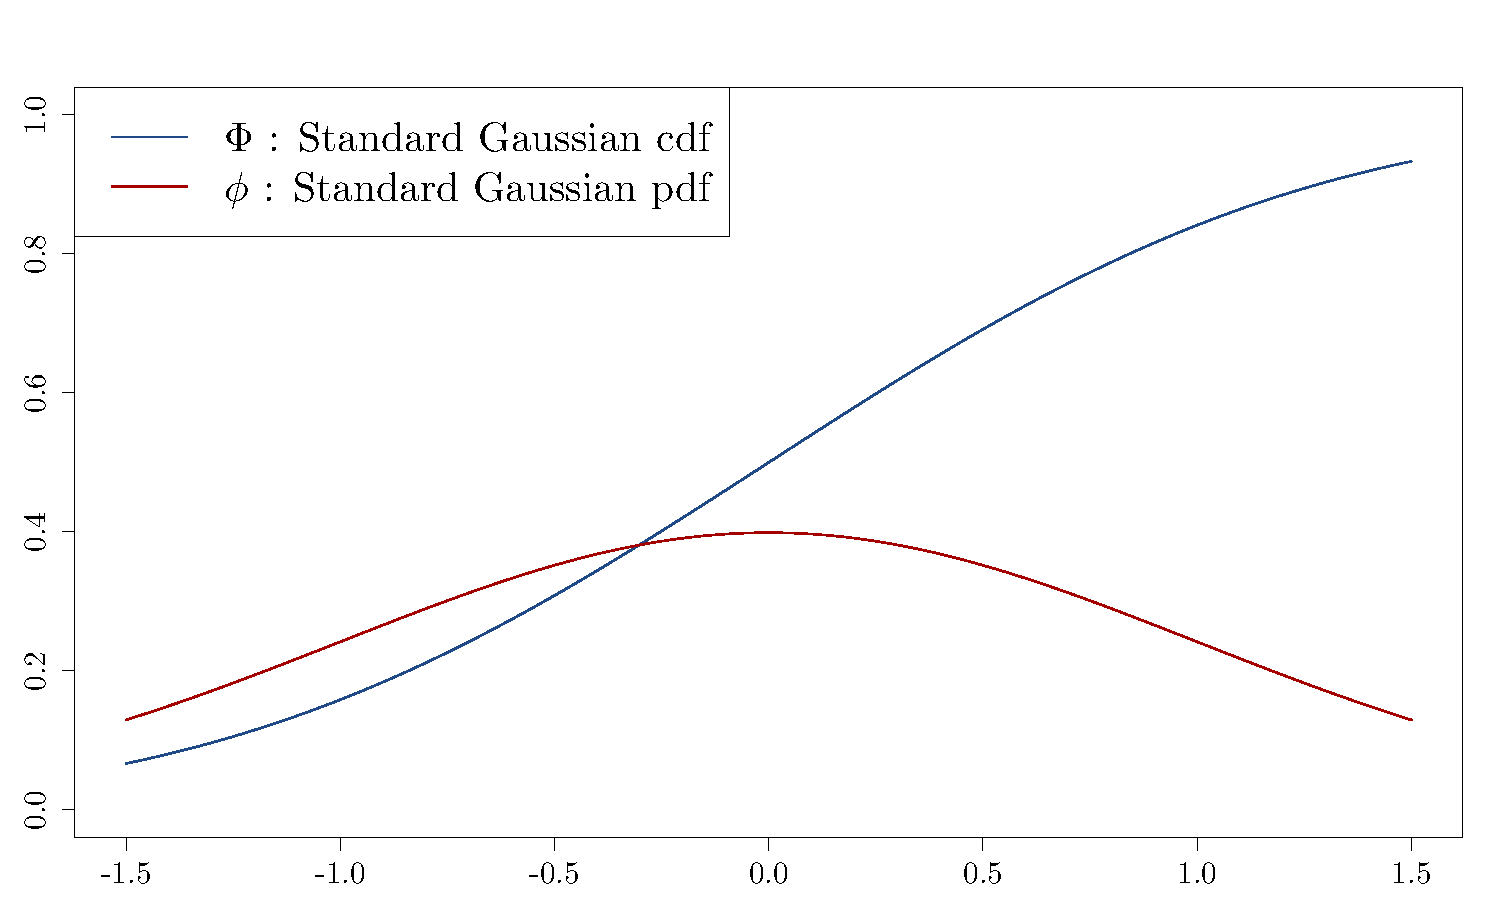
\includegraphics[width=12cm]{figures/exo_optim.pdf}
\end{center}

\end{document}











Given 
\begin{itemize}
	\item the kernel (either exponential, Brownian, squared exponential or Mat\'ern 3/2),
	\item if the process is centred (yes/no),
	\item if the process is stationary (yes/no).
\end{itemize}
\begin{center}
	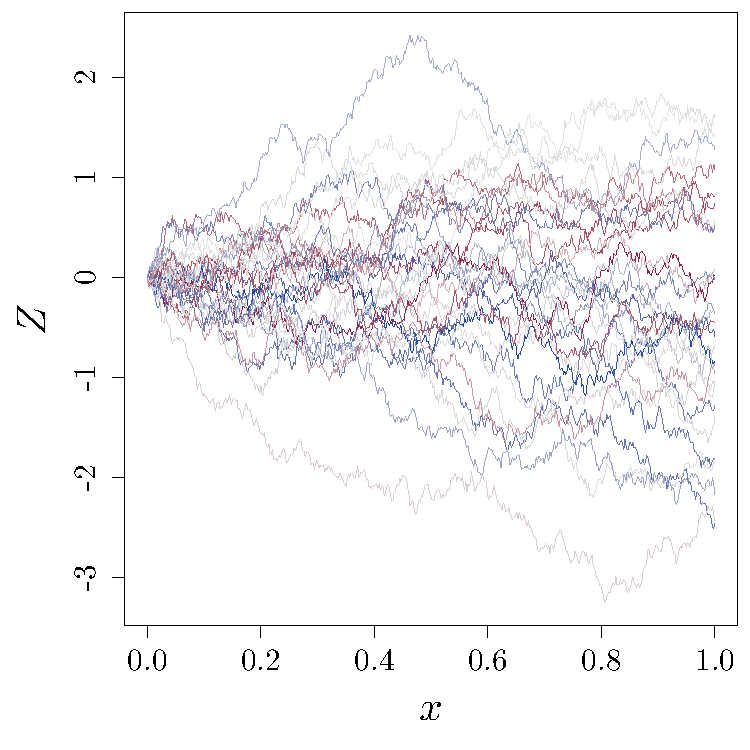
\includegraphics[width=5cm]{figures/GPR_simBrown.pdf} \qquad
	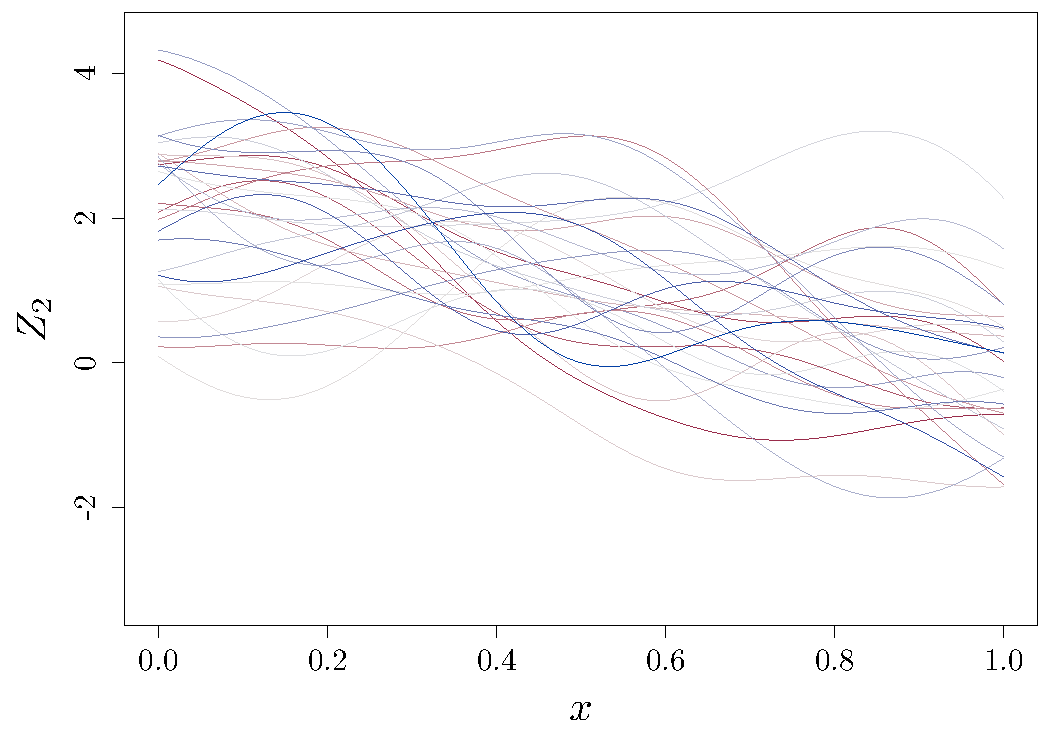
\includegraphics[width=5cm]{figures/GPR_simGauss.pdf}\\
	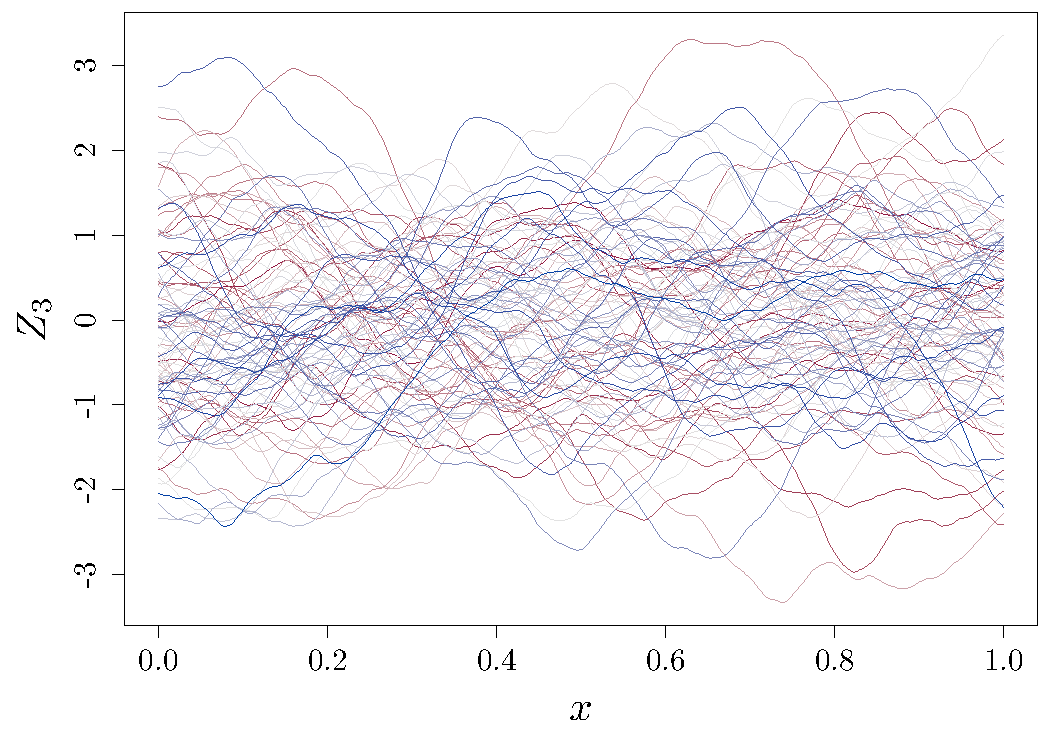
\includegraphics[width=5cm]{figures/GPR_simMat.pdf} \qquad
	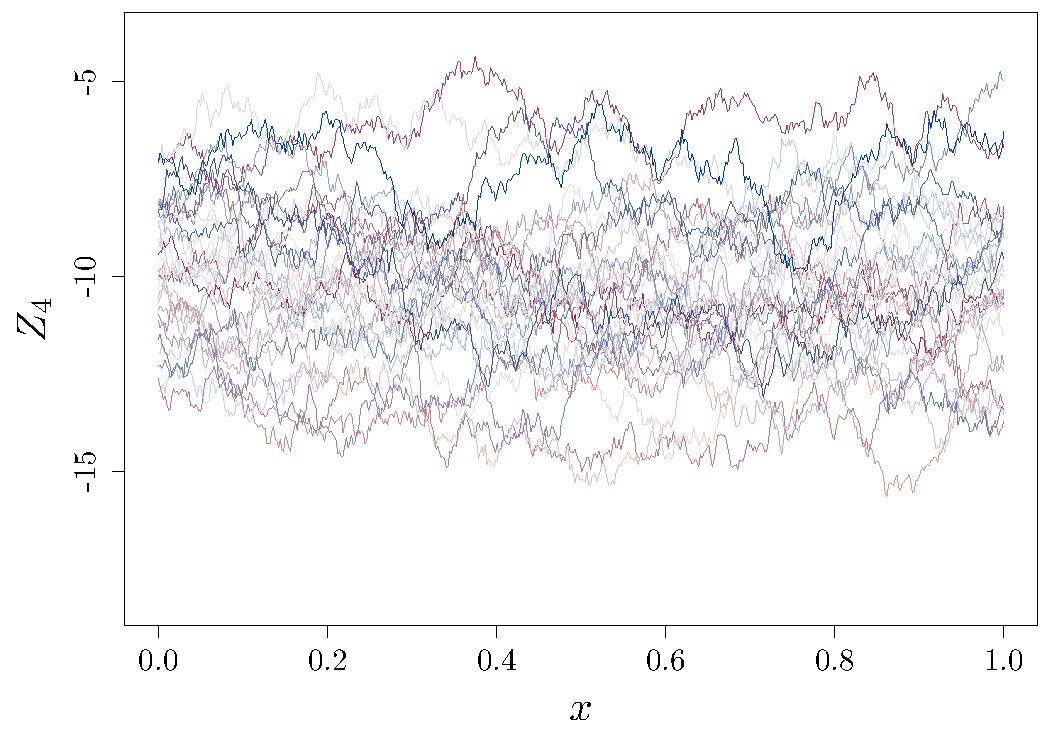
\includegraphics[width=5cm]{figures/GPR_simExp.pdf}
\end{center}
\item{[1 pt]} The figures bellow correspond to samples of a Matern 5/2 kernel with variance parameter $\sigma^2 \in \{0.1, 1, 10, 100 \}$ and with length scale $\theta \in \{0.1,1,10\}$. For each figure, specify the corresponding set of parameters.
\begin{center}
	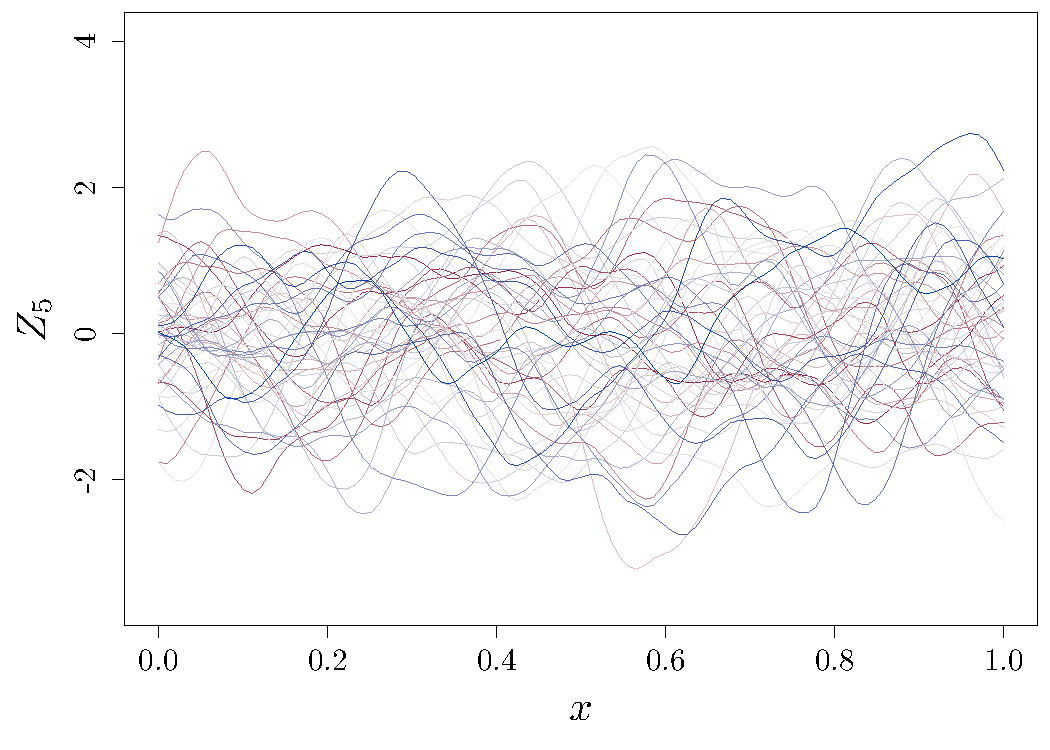
\includegraphics[width=5cm]{figures/GPR_simMat52_1_01.pdf} \qquad
	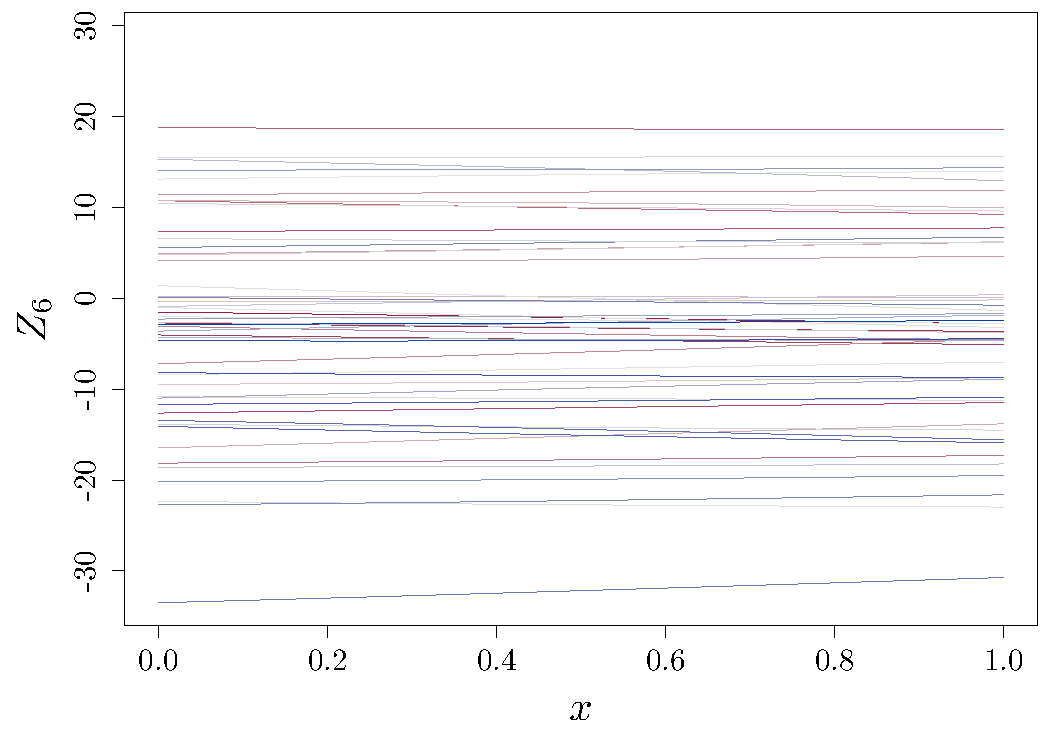
\includegraphics[width=5cm]{figures/GPR_simMat52_100_10.pdf} \\
\end{center}
\item {[1.5 pts]} We are interested in computing the mean value of a function $f$ using no more that 50 observations. What are the main steps you would go through for solving this problem.
\end{enumerate} 

\newpage
%%%%%%%%%%%%%%%%%%%%%%%%%%%%%%%%%%%%%%%%%%%%%%%%%%%%%%%%%%%%%%%%%%%%
%%%%%%%%%%%%%%%%%%%%%%%%%%%%%%%%%%%%%%%%%%%%%%%%%%%%%%%%%%%%%%%%%%%%
\section*{Exercise 2 (7 pts)}
Let us consider the 2-dimensional function: $f(x_{1},x_{2})= x_1 + x_2 + x_1 x_2$.\\

\noindent
The aim is to perform a global sensitivity analysis of $f(X_{1},X_{2})$
where $X_{1}$, $X_{2}$ are independent uniform random variables, 
with $X_1 \sim \mathcal{U} \left[-\frac{a}2,\frac{a}2 \right]$  and  $X_2 \sim \mathcal{U}[-\frac{1}2,\frac{1}2]$,
and $a>0$.\\

\noindent We recall that for a uniform random variable $Z \sim \mathcal{U}[s,t]$, 
we have $\E(Z)= \frac{s+t}2$ and $\var(Z) = \frac{(t-s)^2}{12}$.\\

\begin{enumerate}
\item {[}2 pts{]} By verifying that $X_1$, $X_2$ and $X_1X_2$ satisfy the centering and non-simplification conditions,
show that the Sobol-Hoeffding decomposition of $f(X_1, X_2)$ is simply:
$$\mu_0 = 0, \quad  \mu_1(X_1) = X_1, \quad \mu_2(X_2) = X_2, \quad \mu_{1,2}(X_1, X_2) = X_1X_2$$
\item {[}1.5 pts{]} Compute the partial variances $D_I = \var(\mu_I(X_I))$ for $I = \{1\}, \{2\}, \{1,2\}$ 
and check that the global variance is $D = \var(f(X_1, X_2)) = \frac{1}{12} \left( 1 + \frac{13}{12} a^2 \right)$ 
\item {[}1.5 pts{]} Recall that Sobol indices are defined by $S_I = D_I/D$. Compute $S_1$ and $S_2$, 
and check that $S_1$ (resp. $S_2$) is an increasing (resp. decreasing) function of $a$. Interpretation?\\
\end{enumerate} 

\noindent We now assume that $X_{1}$, $X_{2}$ are independent random variables, with $X_1, X_2 \sim \mathcal{U}[0, 1]$.\\

\begin{enumerate}
\setcounter{enumi}{3}
\item {[}0.5 pt{]} Explain why it is now \textit{wrong} that $\mu_1(X_1) = X_1$.
\item {[}1.5 pts{]} Compute the Sobol decomposition of $f(X_1, X_2)$. 
\end{enumerate}

%%%%%%%%%%%%%%%%%%%%%%%%%%%%%%%%%%%%%%%%%%%%%%%%%%%%%%%%%%%%%%%%%%%%
%%%%%%%%%%%%%%%%%%%%%%%%%%%%%%%%%%%%%%%%%%%%%%%%%%%%%%%%%%%%%%%%%%%%
\section*{Exercise 5: ANOVA kernels (8 pts)}
ANOVA kernels are kernels over $\mathds{R}^d \times \mathds{R}^d$ of the form : $ k(x,y) = \prod_{i=1}^d  \big(1+k_i(x_i,y_i) \big)$, where the $k_i$ are symmetric positive semi-definite functions.

\begin{enumerate}
\item{[1 pt]} Using the results from the course, show that ANOVA kernels are valid covariance functions.
\end{enumerate} 

\noindent We now consider costly-to-evaluate function $f: [0,1]^{10} \to \mathds{R}$, a design of experiment $X$ based on 100 points and the set of observations $F$. The knowledge we have about $f$ is that it is a smooth function that is infinitely differentiable. 

\begin{enumerate}
\setcounter{enumi}{1}
\item{[1 pt]} With such settings, which kernel would you choose and what kind of Gaussian process regression model would you consider (simple Kriging, ordinary Kriging, Universal Kriging).  
\item{[1 pt]} Give the expressions of the mean predictor and of the 95\% confidence intervals.  
\item{[1 pt]} Show that the mean predictor can be interpreted as a sum of $2^d$ functions with increasing interaction order. Does this decomposition coincides with the Sobol decomposition of the mean predictor? Why ?
\item{[1 pt]} Each term of this decomposition can be interpreted as a Gaussian process conditional distribution. Detail which one and deduce some confidence intervals associated to each sub-model.
\item{[2 pts]} According to an expert, the mean value of $f$ is 6 and the interactions of order higher than 2 can be neglected. What changes can you make in the model and in the kernel expression in order to account for these informations ?
\item{[1 pt]} We now consider a particular type for the univariate kernels $k_i$ such that $\int_0^1 k_i(s,x) \, ds = 0$ for all $x \in [0,1]$. Is there a link between the sub-models and the Sobol decomposition in this particular case?
\item[\textbf{bonus:}] Detail how to obtain a kernel $k_i$ such that $\int_0^1 k_i(s,x) \, ds = 0$ using the conditional distribution of a Gaussian process given it has zero integral.
\end{enumerate} 

Consider the kriging of following conditional points:
\[ (x,y) = \begin{cases} (-0.2,-0.2) \\\\ (0.2,0.2) \end{cases}\] with
given range \(\theta=0.2\) and variance \(\sigma^2=0.01\)

\begin{enumerate}
\def\labelenumi{\arabic{enumi}.}
\tightlist
\item
  Use simple kriging equations with exponential covariance kernel to get
  the prediction at \(x=0\).
\end{enumerate}

\textbf{Note:} \[
\left[ \begin{array}{ccc}  a & b \\ b & a   \end{array} \right] ^{-1} = {1 \over {a^2-b^2}} \times \left[ \begin{array}{ccc}  a & -b \\ -b & a   \end{array} \right]
\]

\begin{enumerate}
\def\labelenumi{\arabic{enumi}.}
\setcounter{enumi}{1}
\item
  Evaluate Expected Improvement criterion at \(x=0\).
\item
  Perform the same evaluation for gaussian kernel (with same
  parameters). Compare. Analyse.
\end{enumerate}


\end{document}
